% Author: Animesh Garg
% Date: June 23, 2013

\section{RESULTS}
\label{sec:Results}

We will include quantative comparison 
\begin{figure}[t!]
  \begin{center}
    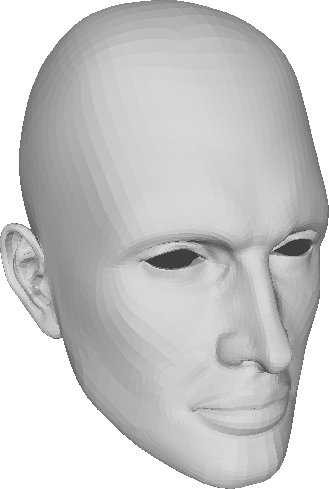
\includegraphics[width=0.65\linewidth]{images/maleHead}
  \end{center}
  \vspace{-10pt}
\caption{ The figure depicts a mesh of a male head. This head is used a test case for evaluating the smallest set grasp points needed for form fixture which also minimize the maximum contact wrench.}
  \vspace*{-10pt}
  \label{fig:maleHead}
\end{figure}

\begin{figure}[t!]
  \begin{center}
    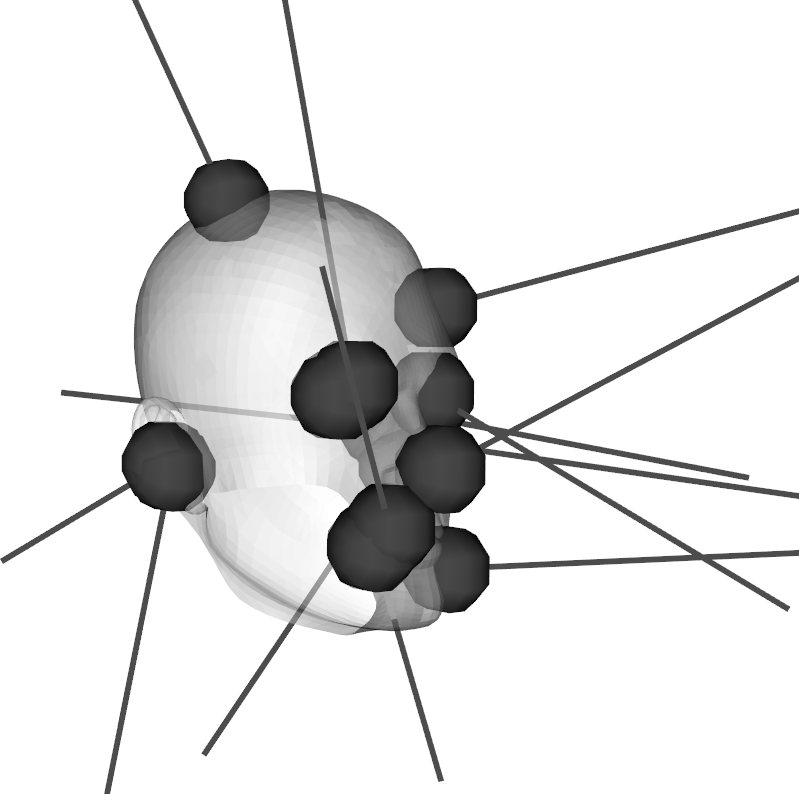
\includegraphics[width=0.75\linewidth]{images/maleHead-graspPoints-v1}
  \end{center}
  \vspace{-10pt}
\caption{ The figure depicts a set of grasp points generated for the aforementioned mesh of a male head. We note that the uniform sampling of candidate contact points results in pathological results. Hence we sample contact points as proposed in \ref{sec:Algorithm}}
  \vspace*{-15pt}
  \label{fig:maleHead-graspPoints}
\end{figure}